%rubber: module pdflatex

\documentclass[11pt,a4paper,variablewidth]{article}

\usepackage[sans]{tcc_doc} % SDP style file
\usepackage[english]{babel}
\usepackage{amssymb,amsmath} % for the math symbols
\usepackage{mdwlist}
\usepackage{geometry}
\usepackage{marginnote}
\usepackage{datetime}
\usepackage{graphicx}
\usepackage{verbatim}
\usepackage{mathtools}
\usepackage{hhtensor}
\usepackage{color}
\usepackage{txfonts}
\usepackage{enumitem}
\usepackage{minted}
\usepackage{tcolorbox}
\usepackage{float}



%\usepackage{stylefiles/fmtcount}
\usepackage{natbib}

\graphicspath{ {images/} }

\usepackage[boxruled,linesnumbered]{algorithm2e}
\usepackage{fmtcount}

\usepackage{array}
\newcolumntype{L}{>{\centering\arraybackslash}m{3cm}}


% TODO:
% 1. Check if all new symbols have been explained when used for the first
% time.
% 2. Check if all symbols are actually being used.
% 3. Check the symbol definitions: rates, numbers, etc. to use the same main letter
% 4. Is there a way to use proper referencing of applicable and reference
% documents?



%%%%%%%%% START OF USER SETTINGS %%%%%%%%%%%%%%%%%%

% Enter here some information needed to fill in the template Title to appear
% on the front pages (will be filled in via the \sdpfrontpage command)
\newcommand{\bigdoctitle}{Distribution of the Rau-Cornwell MSMFS algorithm \xspace}
% Title to go in the "Document Status Sheet" Document number
\newcommand{\docnr}{TCC-CASS-001\xspace}
% Context
\newcommand{\context}{(ASKAPsoft)}
% Revision
\newcommand{\revision}{0.1\xspace}
% Author(s)
\newcommand{\docauthor}{T.J.\ Cornwell\xspace}
% Lead author (goes in the footer)
\newcommand{\leadauthor}{T.J.\ Cornwell\xspace}
% Release date (YYYY-MM-DD)
\newcommand{\docudate}{\today\ \currenttime}
% Document classification
\newcommand{\classification}{Unrestricted}
% Status of the document (draft/final/etc.)
\newcommand{\docstatus}{Released\xspace}

% The definitions below are used for the signature tables in the preamble of
% the document
\newcommand{\firstsigname}{T.J. Cornwell}
\newcommand{\firstsigdesignation}{Author}
\newcommand{\firstsigaffiliation}{TCC}

\newcommand{\secondsigname}{T.J. Cornwell}
\newcommand{\secondsigdesignation}{Lead Consultant}
\newcommand{\secondsigaffiliation}{TCC}

% Table with version numbers
\newcommand{\versiontable}{
  \begin{tabularx}{\textwidth}{|X|X|X|X|}
    \hline
    \bf{Version} & {\bf Date of issue} & {\bf Prepared by} & {\bf Comments}\\
    \hline
    0.1 & 03/04/2018 & T.J. Cornwell & Initial version \\
    \hline
  \end{tabularx}
}

%%%%%%%%%%%%% END OF USER SETTINGS %%%%%%%%%%%%%%%%%%%

% Table with signatures
\newcommand{\signaturetable}[3]{
  \begin{tabularx}{\textwidth}{|X|X|X|}
    \hline
    Name & Designation & Affilitation\\
    \hline
    {#1} & {#2} & {#3}\\
    \hline
    Signature \& Date: & & \\
    & & \\
    & & \\
    \hline
  \end{tabularx}
}



% Table with affiliations
\newcommand{\organisationtable}{
  \begin{center}
    \sffamily{\bf ORGANISATION DETAILS}\end{center}
  \begin{table}[htb]
    \centering
    \begin{tabular}[htb]{|l|l|}
      \hline
      Name & Tim Cornwell Consulting\\
      \hline
    \end{tabular}
  \end{table}
}


%%%%%%%%%%%%%%%%%%%% START YOUR DOCUMENT HERE %%%%%%%%%%%%%%%%%

\newcommand{\subsubsubsection}[1]{\noindent{\bf{#1}}}

%%%% Please DO USE the symbol definitions listed below to preserve
%%%% consistency.

%%%% If you need a new symbol, please add it here. If really want to modify
%%%% one, do so, just take care to do a search-and-replace for the entire document
% Symbol definitions



\begin{document}

% load automatic pages
\tccfrontpage

\sdptableofcontents

% Add here the abbreviations used in your document
\sdplistofabbreviations
\begin{basedescript}{\desclabelstyle{\pushlabel}\desclabelwidth{6em}}
    \item[ASKAP] Australian Square Kilometer Array Pathfinder\vspace{-0.2cm}
    \item[ARL] Algorithm Reference Library\vspace{-0.2cm}
    \item[FFT] Fast Fourier Transform\vspace{-0.2cm}
    \item[FLOP] Floating Point Operations \vspace{-0.2cm}
    \item[FLOPS] Floating Point Operations per Second \vspace{-0.2cm}
    \item[FoV] Field of View\vspace{-0.2cm}
    \item[MS-MFS] Multi-Scale Multi-Frequency Synthesis\vspace{-0.2cm}
    \item[MAM] Multi-Scale Multi-Frequency Synthesis\vspace{-0.2cm}
    \item[PSF] Point Spread Function \vspace{-0.2cm}
    \item[SDP] Scientific Data Processor\vspace{-0.2cm}
    \item[SKA] Square Kilometre Array\vspace{-0.2cm}
%    \item[] \vspace{-0.2cm}
\end{basedescript} 

\newcommand{\nuno}{{\left(\frac{\nu}{\nu_0}\right)}}
\newcommand{\dnuno}{{\left(\frac{\nu-\nu_0}{\nu_0}\right)}}

\newcommand{\dg}{^\dag}
\newcommand{\X}{\vec{x}}
\newcommand{\Xd}{\vec{{x}^\dag}}
\newcommand{\B}{\vec{b}}
\newcommand{\Bd}{\vec{b^\dag}}
\newcommand{\V}{\vec{V}}
\newcommand{\Vd}{\vec{V^\dag}}
\newcommand{\A}{{\tens{A}{}}}
\newcommand{\Ad}{{\tens{A^\dag}{}}}
\newcommand{\F}{{\tens{F}{s}}}
\newcommand{\Fd}{{\tens{F^\dag}{}}}
\newcommand{\He}{{\tens{H}{}}}
\newcommand{\Sa}{{\tens{S}{}}}
\newcommand{\Sd}{{\tens{S^\dag}{}}}
\newcommand{\Sna}{\tens{{S_{\nu}}{}}}
\newcommand{\Snd}{\tens{{S_{\nu}^\dag}{}}}
\newcommand{\T}{{\tens{T}{}}}
\newcommand{\W}{{\tens{W}{}}}
\newcommand{\Wd}{{\tens{W^\dag}{}}}
\newcommand{\Pb}{{\vec{P}}}

%\newcommand{\Wim}{{\tens{W^{im}}}}
%\newcommand{\Wimd}{{\tens{{W^{im}}^\dag}}}
%\newcommand{\Wnt}{{\tens{W^{\rm {mfs}}_t}}}
%\newcommand{\Wntd}{{\tens{{W^{\rm {mfs}}_t}^\dag}}}
%\newcommand{\Wnp}{{\tens{W^{\rm mfs}_p}}}
%\newcommand{\Wnpd}{{\tens{{W^{\rm mfs}_p}^\dag}}}
%\newcommand{\Wnq}{{\tens{W^{\rm mfs}_q}}}
%\newcommand{\Wnqd}{{\tens{{W^{\rm {mfs}}_q}^\dag}}}
%\newcommand{\Wimn}{{\tens{W^{im}_{\nu}}}}
%\newcommand{\Wimnd}{{\tens{{W^{im}_{\nu}}^\dag}}}

\newcommand{\Wim}{{{\W^{\rm im}}}}
\newcommand{\Wimd}{{{{\W^{\rm im}}^\dag}}}
\newcommand{\Wnt}{{{\W^{\rm {mfs}}_t}}}
\newcommand{\Wntd}{{{{\W^{\rm {mfs}}_t}^\dag}}}
\newcommand{\Wnp}{{{\W^{\rm mfs}_p}}}
\newcommand{\Wnpd}{{{{\W^{\rm mfs}_p}^\dag}}}
\newcommand{\Wnq}{{{\W^{\rm mfs}_q}}}
\newcommand{\Wnqd}{{{{\W^{\rm {mfs}}_q}^\dag}}}
\newcommand{\Wimn}{{{\W^{\rm im}_{\nu}}}}
\newcommand{\Wimnd}{{{{\W^{\rm im}_{\nu}}^\dag}}}

\newcommand{\wnt}{{w_{\nu}^t}}
\newcommand{\wnq}{{w_{\nu}^q}}
\newcommand{\wntq}{{w_{\nu}^{t+q}}}
%\newcommand{\Wntn}{{\tens{w^{\rm mfs}_{t,\nu}}}}
%\newcommand{\Wntnd}{{\tens{{w^{\rm mfs}_{t,\nu}}^\dag}}}
%\newcommand{\Wnpn}{{\tens{W^{\rm mfs}_{p,\nu}}}}
%\newcommand{\Wnpnd}{{\tens{{W^{\rm mfs}_{p,\nu}}^\dag}}}

\newcommand{\pd}{{\partial}}
\newcommand{\mi}{{m_{I}}}
\newcommand{\R}{{R}}
\newcommand{\Rd}{{R^\dag}}
\newcommand{\I}{{\vec{I}}}

\newcommand{\Nt}{N_{\rm Taylor}}
\newcommand{\Ns}{N_{\rm scales}}
\newcommand{\Nc}{N_{\rm chan}}
\newcommand{\Np}{N_{\rm pix}}
\newcommand{\Nf}{N_{\rm Facet}}

\newcommand{\MAM}{M\&M}

\newcommand{\ARL}{ARL}


\sdplistoffigures

\sdplistoftables

% Add here the executive summary
\sdpsummary

The MSMFS algorithm is integral to the data processing for ASKAP and SKA. The inner loops for ASKAP continuum processing use the Multi-Scale Multi-Frequency Synthesis (MSMFS, also \MAM\footnote{SDP adopted this name since it is easier to say.}) to model the changing structure of the source over frequency. By synthesising across frequency, the imaging performance of the telescope can be improved.

\MAM\ consists of a major cycle that compares the current model with the visibility data, and a minor cycle that deconvolves in (RA, Dec, scale, moment) space. The major cycle is composed to gridding, degridding, and FFT steps and has seen the most effort in optimisation. The minor cycle of \MAM\ consists of a modified and extended CLEAN in image space. This is currently executed in a single thread and can constitute a significant overhead in that processing is blocked until this CLEAN finishes.

The amount of processing in typical use of \MAM\ is comparable to that in the invert and predict steps. Hence since the \MAM\ step is currently serial, it will inevitably result in a bottleneck. The cure is to reduce the amount of work in \MAM\ and and/or distribute the work across multiple workers.

We investigate the various ways that the distribution can be performed.

\newpage

\subsection*{Reference Documents}

The following documents are referenced in this document. In the event of
conflict between the contents of the referenced documents and this document,
\emph{this document} shall take precedence.

 \begin{center}
 \begin{tabularx}{\textwidth}{|l|X|}
     \hline
     \bf{Reference} & \bf{Reference}\\
     \bf{Number} & \\
     \hline
   {\bf [RD01]} & \url{http://www.astron.nl/casacore/trunk/casacore/doc/notes/229.html}\\
   {\bf [RD02]} & Imager.cc C++ source, CASA source code SVN revision 30821, \url{https://svn.cv.nrao.edu/svn/casa/trunk}\\ 
   {\bf [RD03]} & Parameterized deconvolution for wide-band radio synthesis imaging, Urvashi Rao Venkata, 2010, PhD thesis\\
   {\bf [RD04]} & Cornwell, T. J. (2008). Multi-Scale CLEAN deconvolution of radio synthesis images. IEEE Journal of Selected Topics in Sig. Proc., 2, 793–801.\\
   {\bf [RD05]} & Junklewitz, H., Bell, M. R., and Ensslin, T. (2015). A new approach to multifrequency synthesis in radio interferometry. Astronomy \& Astrophysics, 581, A59. http://doi.org/10.1051/0004-6361/201423465 \\
	{\bf [RD06]} & Rau, U., \& Cornwell, T. J. (2011, June 14). A multi-scale multi-frequency deconvolution algorithm for synthesis imaging in radio interferometry. arXiv.org. EDP Sciences. http://doi.org/10.1051/0004-6361/201117104   \\
	{\bf [RD07]} & Bhatnagar, S., Rau, U., \& Golap, K. (2013). Wide-field wide-band Interferometric Imaging: The WB A-Projection and Hybrid Algorithms. The Astrophysical Journal, 770(2), 91. http://doi.org/10.1088/0004-637X/770/2/91 \\
	{\bf [RD08]} & Cornwell, T.J. (2016), Implementation of the Rau-Cornwell MSMFS algorithm, TCC-SDP-151123-2. \\
	\hline
 \end{tabularx}
\end{center}

\pagebreak
\section{Purpose of the document}


The purpose of this document is to describe options for distributing the minor cycle of the Multi-Scale MultiFrequency Synthesis algorithm, as implemented in ASKAPsoft,.

\section{Scope of the document}

The scope includes only the published Multi-Scale, Multi-Frequency algorithms, existing implementations, and inclusion in the ASKAPsoft processing pipelines. Only the minor cycle of that algorithm is addressed. In addition, the many possible threading possibilities are not explored.

\clearpage

\section{\MAM\ algorithm in ASKAPsoft}

The \MAM\ algorithm implementation has been discussed extensively in RD08. We use the same terminology and symbols.

The (serial) minor cycle from the Urvashi-Cornwell algorithm [RD03, RDO6] is shown below in both pseudo-code (Algorithm \ref{alg:minor_cycle_UC2011}) and python (Figure \ref{fig:minor_cycle_python}).

\begin{algorithm}
%\scriptsize
  \SetLine
  \linesnumbered
  \dontprintsemicolon
  \KwData{input : number of Taylor-terms $\Nt $, number of scales $\Ns $}
  \KwData{input : image noise threshold, $\sigma_{\rm thr}$, loop gain $g$}
  \KwData{input : scale basis functions : $\I^{\rm shp}_s ~ \forall s\in\{0,\Ns -1\}$}
  \KwResult{model coefficient images : $\I^{\rm m}_{t}~ \forall t\in\{0,\Nt -1\}$}
  \Repeat { Peak residual in $\vec{I}^{\rm res}_{{0}\atop{0}} < f_{\rm limit} $ } 
    {
     \For{$s \in \{0,\Ns $-$1\}$}
     {
       {
          Construct $\I^{\rm rhs}_s$, an $\Nt \times 1$ vector from $\I^{\rm res}_{{s}\atop{t}} ~~\forall ~ t \in \{0,\Nt $-$1\}$\;
          Compute principal solution $\I^{\rm sol}_s = [{\He^{\rm peak}_s}^{-1}] \I^{\rm rhs}_s$\;
          Fill solution $\I^{\rm sol}_s$ into model images $\forall t$ : $\I^{\rm m,sol}_{{s}\atop{t}}$
       }
     }
     Choose $\I^{\rm m}_{{p}\atop{t}} = max\{\I^{\rm m,sol}_{{s}\atop{t=0}},~\forall~s\in\{0,\Ns $-$1\}\}$ \;
       \For{$t \in \{0,\Nt -1\}$}
       {
        Update the model image : $\I^{\rm m}_t = I^{\rm m}_t + g ~[ \I^{\rm shp}_{p} \star \I^{\rm m}_{{p}\atop{t}}]$ \;
        }
       \For{$t \in \{0,\Nt -1\}$}
       {
        \For{$s \in \{0,\Ns $-$1\}$}
	{
          Update the residual image : $\I^{\rm res}_{{s}\atop{t}} = \I^{\rm res}_{{s}\atop{t}} - g ~\sum_{q=0}^{\Nt -1}[\I^{\rm PSF}_{{sp}\atop{tq}} \star \I^{\rm m}_{{p}\atop{t}}]$\;
	}
       }
    }
\caption[Minor cycle of \MAM\ Algorithm]
         {Minor cycle of \MAM}\label{algo:ASKAP}
\label{alg:minor_cycle_UC2011}
\end{algorithm}

\begin{figure}
\begin{tcolorbox}
\inputminted{python}{minor_cycle.py}
\end{tcolorbox}
\caption{Minor cycle in python}
\label{fig:minor_cycle_python}
\end{figure}

\clearpage

\pagebreak
\section{Scale of problem}

To study the scale of the problem without running large numbers of simulations, we have adapted the SKA Performance Model to ASKAP processing. The PM is a python library and accompanying Jupyter notebooks. The various steps in SKA processing have been expressed using the symbolic math capabilities of sympy. This allows both evaluation of a particular configuration of processing as a function of a range of parameters. We have developed a branch of the code specially adapted to ASKAP processing.

The SKA ICAL pipeline performs continuum imaging and self-calibration. A typical case for ASKAP is shown in figure \ref{fig:processing_histogram}. 

\begin{figure}[htb]
  \centering
  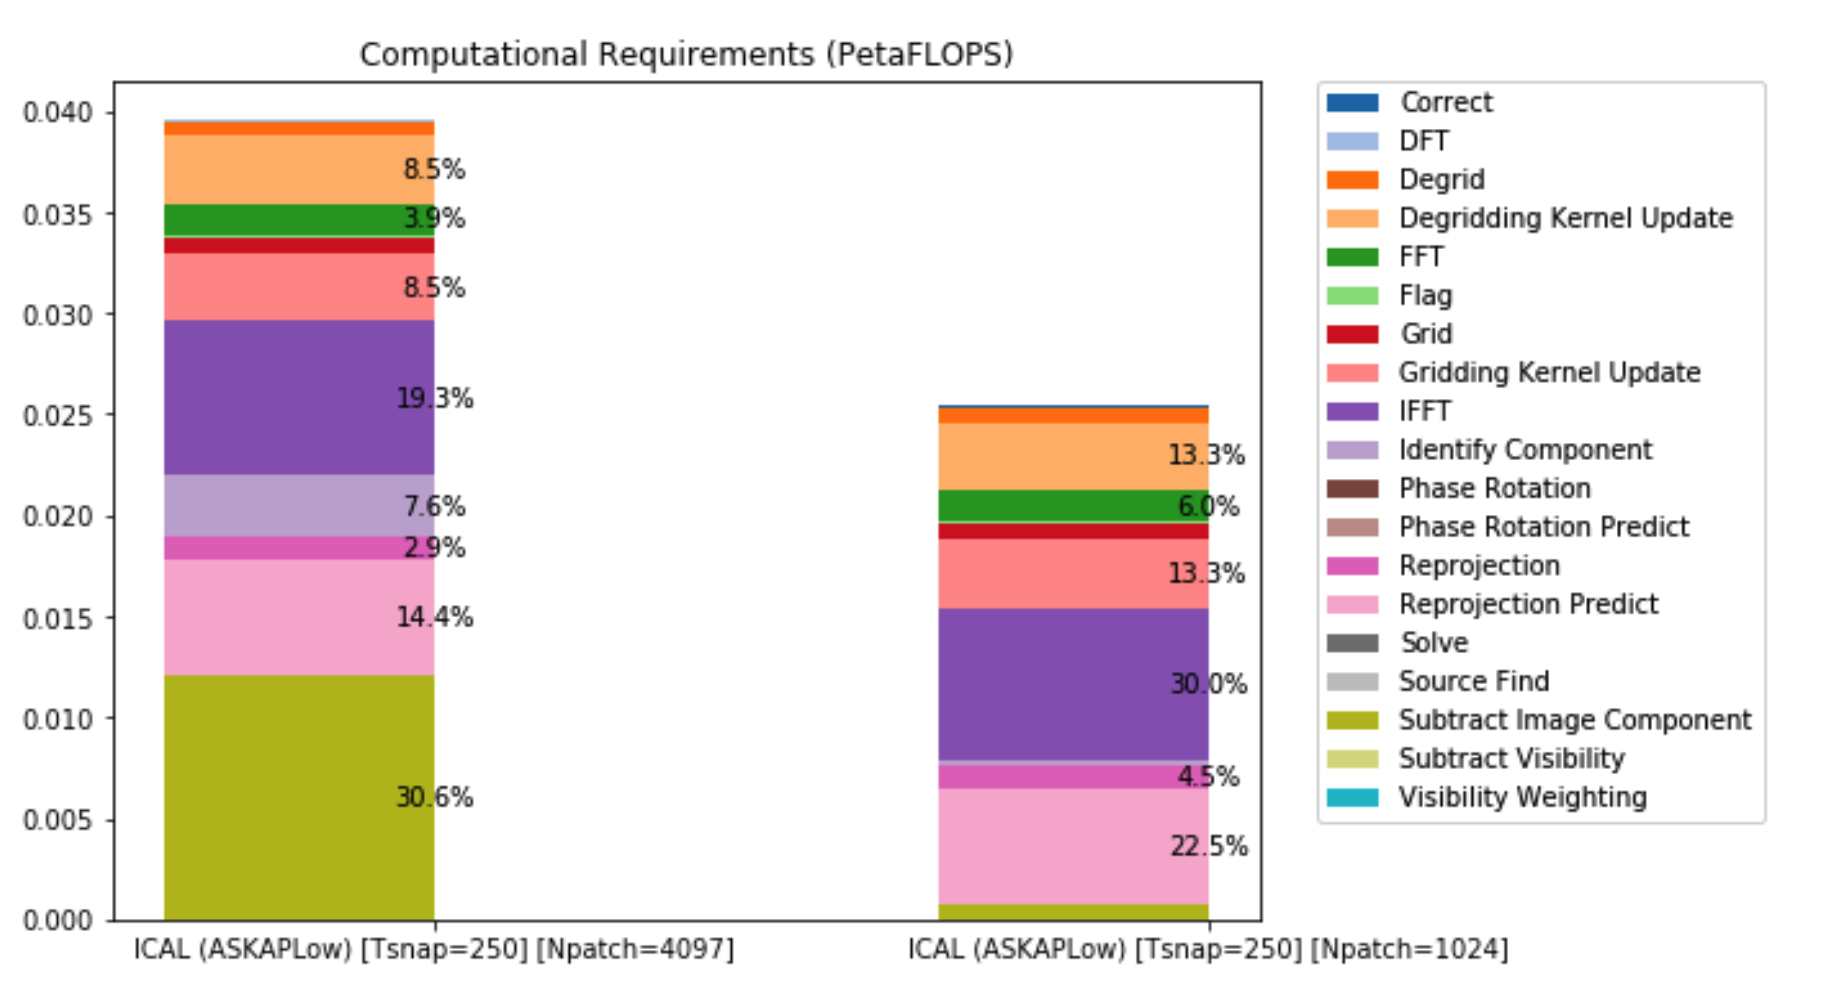
\includegraphics[width=\textwidth]{./processing_histogram.png}
  \caption{Estimation of the cost of processing steps from the SKA Performance Model as adapted to ASKAP. Left column is for large PSF patch size, right is for patch size of 512, which is the recommended value for ASKAP processing.}
  \label{fig:processing_histogram}
\end{figure}

Identify Component in the SKA model corresponds to line 2 - 6 in \ref{alg:minor_cycle_UC2011}, and Subtract Image Component to lines 7 - 15. The other parts of the processing in the histogram do distribute with reasonably high efficiency. 

The minor cycle is currently purely serial and therefore constitutes a loss of processing efficiency in a parallel processing context. For N processors, and with a fraction p being amenable to parallelisation, Amdahl's law constrains the maximum speedup to be:

\begin{equation}
S = \frac{1}{(1-p) + \frac{p}{N}}
\end{equation}

The resulting curves are shown in figure \ref{fig:amdahl}. 

The fraction of processing, $p$, for \MAM\ is about 4 \%. Thus the maximum possible speedup of the ICAL pipeline is about 25.
\begin{figure}[htb]
  \centering
  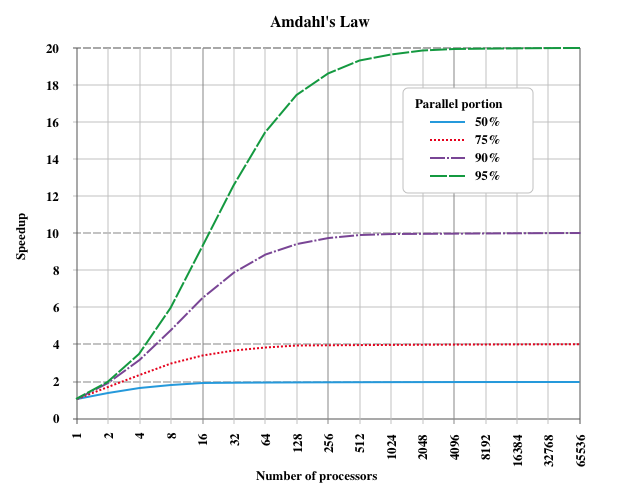
\includegraphics[width=\textwidth]{./AmdahlsLaw.png}
  \caption{Amdahl's law for various fractions of parallel portion.}
  \label{fig:amdahl}
\end{figure}

\clearpage

\pagebreak
\section{Distribution}
\label{sec:distribution}

In this section, we discuss the opportunities for distribution of the inner loop over multiple processing nodes.

The axes of the inner loop are (RA, Dec, Scale, Moment). The numerical ranges of these parameters are as follows:
\begin{description}
\item[RA, Dec] The image sizes for ASKAP are typically 4k x 4k or less. For SKA, numbers are much larger, up to 100k x 100k.
\item[Scale] Typically 3 - 5 scales are used, in a roughly geometric progression such as [0, 3, 10, 30, 100].
\item[Moment] Between 3 and 5 (frequency) moments are typical.
\end{description}

Distributing over scale will at most gain a factor of order 5. The network costs will be very significant. 

More opportunity for distribution lies in the spatial axes. Spatially the coupling occurs for two reasons: the point spread function and the MS blobs. The point spread function can usually be assumed to be sufficiently well-behaved that updating of the residuals is only need in a limited neighbourhood. This statement is scale dependent and larger scales will inevitably show more coupling. It will be necessary to deal with components close to the partition boundary. Thus we will require enforcing some continuity constraint at the partition boundaries. There are a number of ways of doing so. We consider each of these in order of increasing complexity:

\begin{description}
\item[S1. Partition into sub-images]

Divide the image space into a number of disjoint partitions and clean each separately. The drawback to this approach is that large scales close to the boundaries will be penalised, leading to discontinuities in the final image.

\item[S2. Overlap the partitions]

To avoid the penalisation of large scales in S1, each partition could be extended with a suitably sized guard band. At the end of the minor cycle, neighbours could be smoothly interpolated. 

\item[S3. Message passing inside the minor loop]

To avoid conflicts between components found in the overlap region, we could allow the neighbours to communicate every component found. We could partition as in S2 and communicate components found during the minor cycles, either peer-to-peer or to a central broker such as the master. Overlap by at least the largest scale size is required.

Each worker can check to see if a component overlaps with another worker or set of workers. If so, the component can be sent peer-to-peer or via the master. In theory MPI offers mechanisms for such communication but some experimentation might be necessary.

A message would be a flux value[scale, moment], a direction, and a shape, plus some ancillary information such as peak residual, taking O(100) bytes. For scaling, the communication of update events must occur in the same or less time as the worker execution times. The rate of overlap events is proportional to the fraction of the total image space that is subject to overlaps.

\end{description}

S1 and S2 are relatively minor changes and can be implemented and tested with a moderate amount of effort. S3 is considerably more complex to implement and might be subject of the vagaries of MPI. 

\subsection{Data movement for S1, S2}
\label{sec:data_movement}

In ASKAPsoft, at the end of the major cycle the different frequency residual images are sent to the master and combined into the residual frequency cubes. In the current single-threaded approach in ASKAPsoft, the residual images (per Taylor term) and PSF are then deconvolved on the master. Thus there are two synchronisation points: one to assemble the Taylor term cubes and one to await the end of the deconvolution.

In options S1 and S2, the simplest change would be to still combine the image planes on the master but to extract the patch residual images and PSF and distribute those to the workers. Each worker would then apply \MAM\ to it's patch and return the resulting deconvolved image. The entire data flow to the master would be:

\begin{equation}
	R_{IO,{to\ master}} = \Np * \Nc
\end{equation}

Alternatively, instead of the data flow being centralised on the master, the workers could either broadcast the entire image of their frequency term to all workers or each worker could send just the appropriate patch of frequency to each worker.

\begin{equation}
	R_{IO,{pair-wise}} = {\Np/\Nf} * \Nc * \Nf
\end{equation}

Thus the data flow is the same in both cases but is bottlenecked to the master in the first approach. 

The other important factor to consider is the working set size in both cases. In the 
${to\ master}$ approach the memory required in the master is significantly larger because the
entire image cube has to be assembled before distribution to the workers

\subsection{Overlaps and edge effects}

S1 and S2 inevitably create seams in the resulting images where the deconvolution has been performed from different pixels either side of the seam. Making the seam narrow is unlikely to be satisfactory since even for the Hogbom clean the discontinuity will lead to different deconvolution either side of the seam. For the MultiScale clean, the same effect will occur at least on all scales in the deconvolution. Thus we can expect that the taper should be extend over more pixels than the largest scale.

Some possible tapering functions are shown in Figure \ref{fig:tapers}. The simplest is simple addition or averaging, here shown as 'flat'. We improve by using a linear interpolation but this shifts discontinuities into the first derivative. The well-known Tukey filter removes these discontinuities by apply a cosine-taper, thus ensuring that only the second derivative is substantial. The computational cost in using the Tukey filter is negligible so we recommend always using it in preference to the flat of linear tapers.

The loss of efficiency due to the overlaps is non-negligible:

\begin{equation}
\epsilon_{overlap} = \left(\left(N_{pixel} - N_{facets} N_{overlap}\right)/N_{pixel}\right)^2
\end{equation}

For a typical ASKAP case, we would need about 2048 pixels on a side, 8 facets on a side and an overlap of 32, say. For this example, the efficiency due to overlap is $(2048 - 256)/2048) = 0.875$. Increasing the overlap by a factor of two to 64, the efficiency is 0.75. However, we can expect to gain much more than this factor by distribution so we regard this level of inefficiency as acceptable.

\begin{figure}[htb]
  \centering
  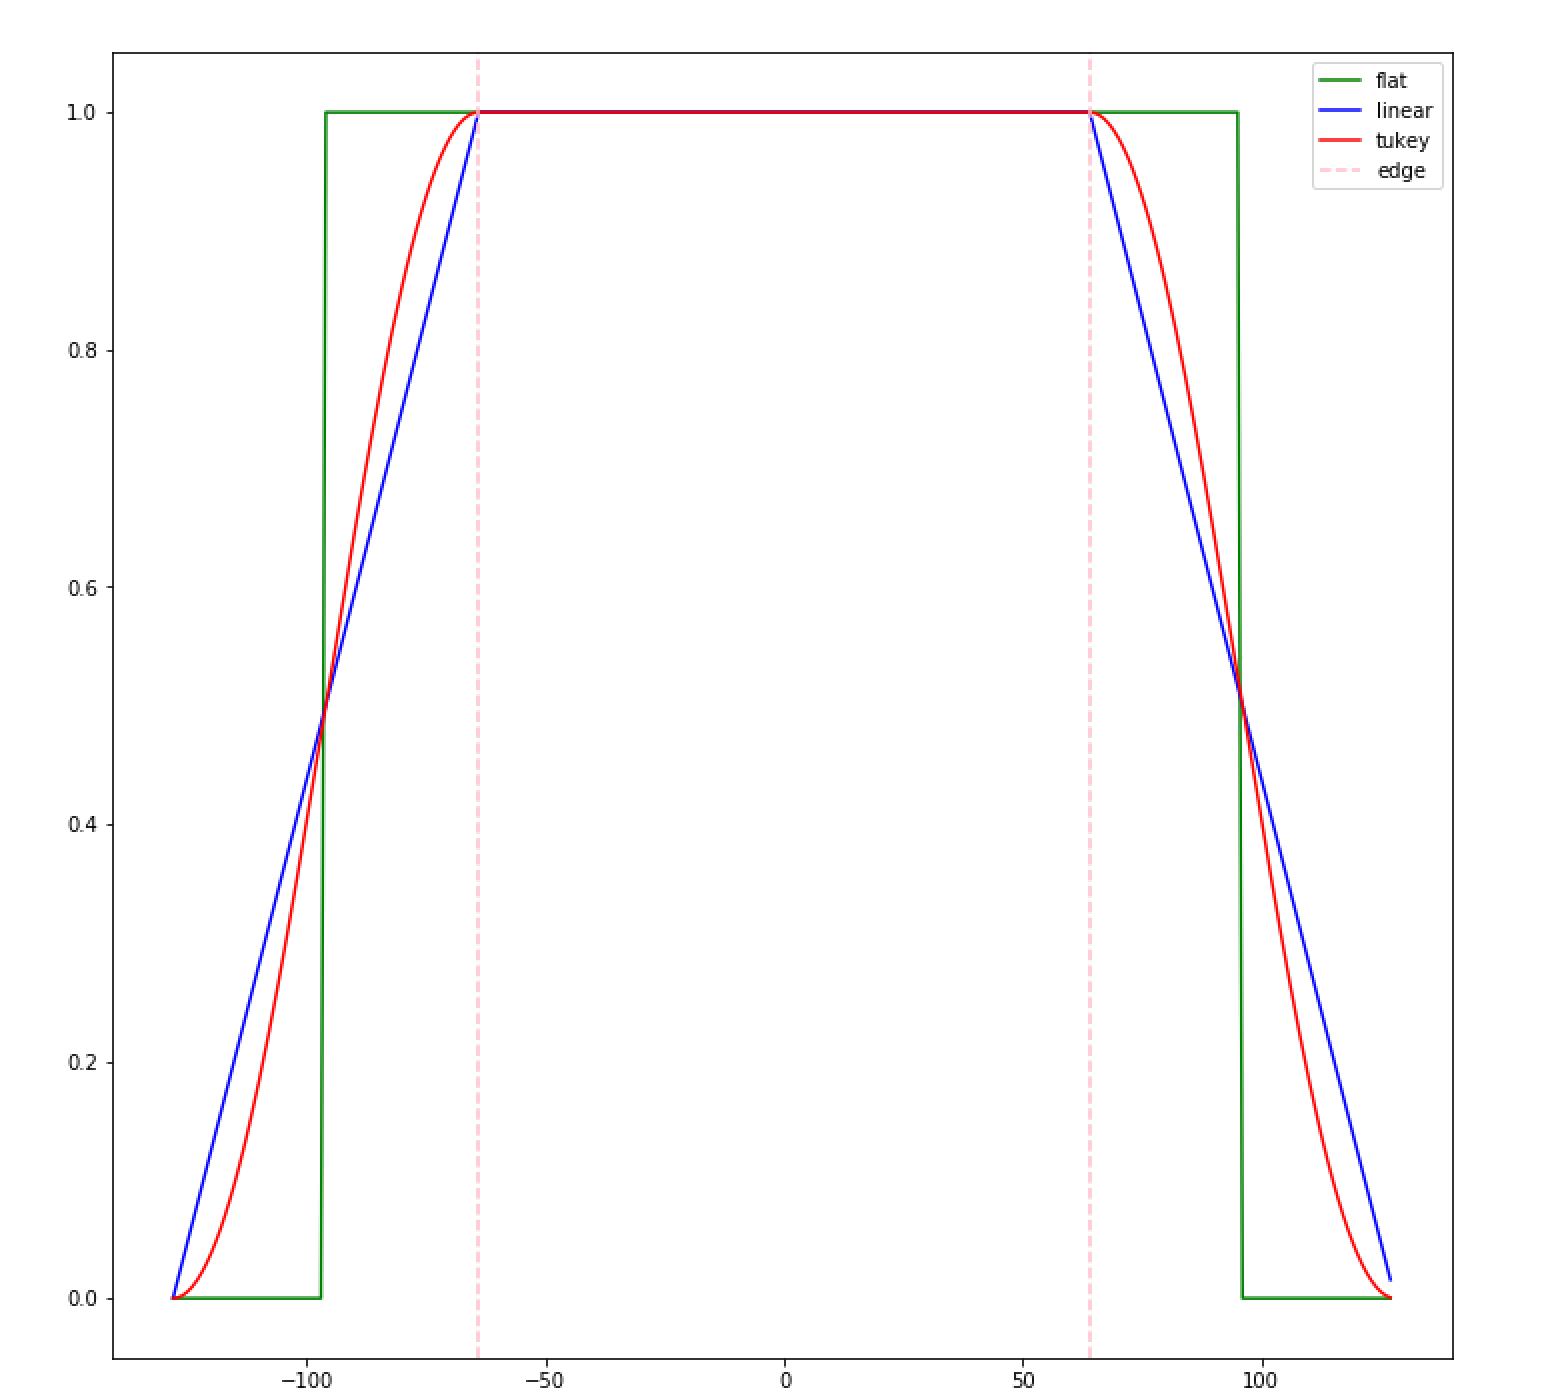
\includegraphics[width=\textwidth]{./tapers.png}
  \caption{Tapers for feathering facet images. The vertical pink lines show the where the overlaps start. This is for 256 pixels and overlap of 64. For this case, the efficiency is roughly $(64/256)^2 = 1/16$}
  \label{fig:tapers}
\end{figure}

\subsection{Load balancing}

The primary cause of load in-balance is that different sub-images will have different numbers of sources and hence different elapsed time for deconvolution. In the graph-based approach used in the \ARL\ this is somewhat mitigated by the intrinsic flexibility of the graph-based work allocation. In MPI, it is possible that some explicit load-balancing may be required. We therefore provide some analysis of the need for load balancing.

If the image is made with a guard band of one or two primary beams, the outermost sub-images will mostly have weak sources and require little deconvolution initially. For the example above of 8 by 8 sub-images, about 16 will have substantial flux to deconvolve. This means that at the beginning of a major/minor cycle algorithm, the maximum scaling is about 16, although we divided the image into 64 sub-images. Using smaller sub-images by a factor of two would bring this scaling limit up to about 64. Essentially the scaling is determined by the number of sub-images we can define across the primary beam.

We can improve on this rough argument by some straightforward modeling. To a reasonable approximation, the processing time for a given sub-image will be proportional to the fraction of a flux in that sub-image. For a given model of the sky, we can calculate the fraction of time taken for each sub-image\footnote{See section \ref{sec:simulations} for more details of the simulations}. We illustrate that point in figures \ref{fig:fractions_without_pb}, \ref{fig:fractions_with_pb}, and \ref{fig:fractions_clipped_image}. The first plot is a realistic astronomical field constructed from the S3-SEX catalog, selected for all sources brighter than 10uJy/beam. The curve shows the fraction of flux per sub-image against rank of that flux. The slope comes from the logN/logS statistics of the S3-SEX catalog. The peak value shows roughly the processing for the worst sub-image. This provides an upper bound on the scaling possible. The variable nproc is an estimate for the number of processors derived by dividing the total amount of processing by the peak value needed.

The next plot (figure \ref{fig:fractions_with_pb}) shows the effect of the ASKAP (single) primary beam. Most sub-images do not require cleaning and all the processing goes to the brightest fields. As processing proceeds thorough a number of major cycles, the brightest sources are been removed and eventually there remains a sea of sources spread other the primary and into the primary beam side-lobes. At this point, we can model the flux as simply by clipping the image with the primary beam at some maximum brightness such as 1mJy. The resulting scaling shown in figure \ref{fig:fractions_clipped_image} is then better balanced.

So, to summarise, we expect the scaling to be poor for the initial major cycles (typically $\sim 5$ for 16 facets per axis) where the brightest sources in the main lobes are removed, but it will improve (typically to $\sim 50$) as the cleaning goes deeper. Since the number of weak sources is much greater we can expect the scaling to be close to that on figure \ref{fig:fractions_clipped_image}

\begin{figure}[H]
  \centering
  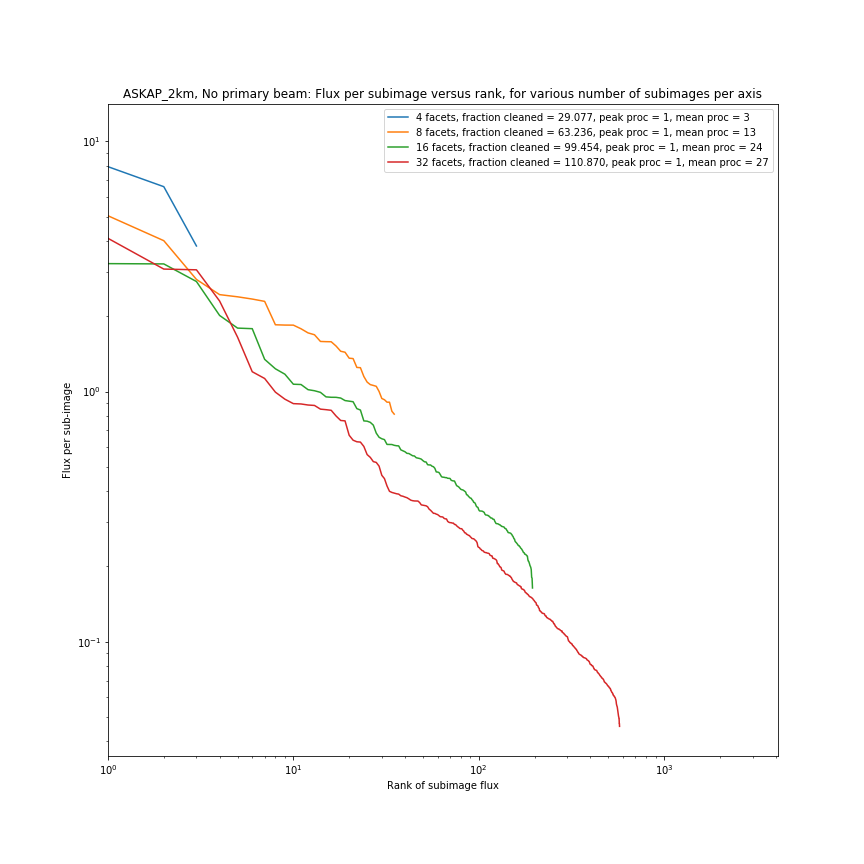
\includegraphics[width=\textwidth]{./fluxes_without_pb_ASKAP_2km.png}
  \caption{Integrated sub-image flux versus rank, for realistic image (constructed from S3-SEX) without a primary beam applied. Scales are [0, 3, 10], and the overlap is 16 pixels. The slope for all curves is mainly due to the statistics of image which is derived from radio source LogN/LogS relationship.}
  \label{fig:fluxes_without_pb}
\end{figure}

\begin{figure}[H]
  \centering
  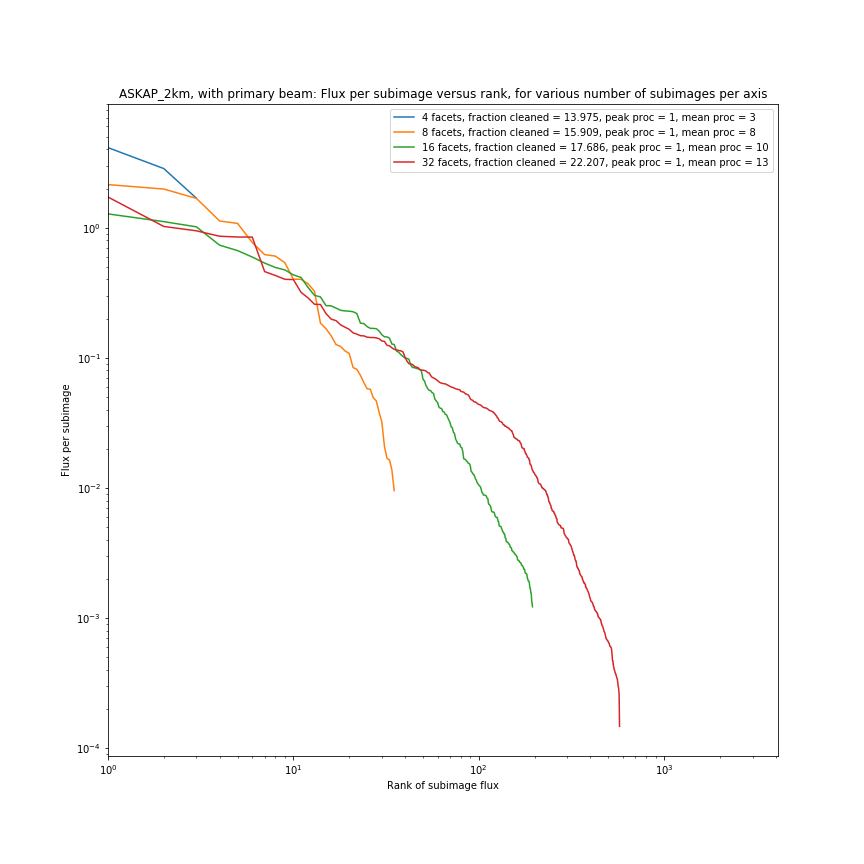
\includegraphics[width=\textwidth]{./fluxes_with_pb_ASKAP_2km.png}
  \caption{Integrated sub-image flux versus rank, for realistic image (constructed from S3-SEX) with a primary beam applied. Scales are [0, 3, 10], and the overlap is 16 pixels. Compared to figure \ref{fig:fluxes_without_pb}}, the primary beam application shifts the high rank sub-images lower in flux.
  \label{fig:fluxes_with_pb}
\end{figure}

\begin{figure}[H]
  \centering
  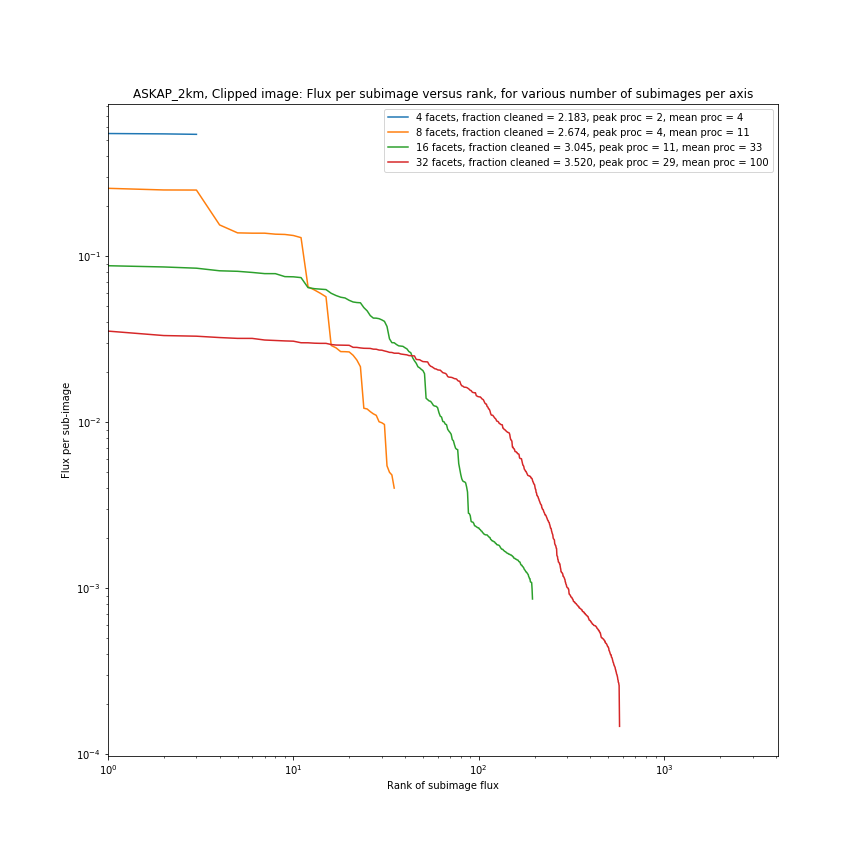
\includegraphics[width=\textwidth]{./fluxes_clipped_image_ASKAP_2km.png}
  \caption{Integrated sub-image flux versus rank for various numbers of sub-images, for realistic image (constructed from S3-SEX) with a primary beam applied and then clipped at 1mJy/beam. Scales are [0, 3, 10], and the overlap is 16 pixels. There are now no bright sources left.}
  \label{fig:fractions_clipped_image}
\end{figure}

To get the overall scaling curve we must sum the work required for a sequence of major cycles going successively deeper. The thresholds start at 0.1 Jy and diminish by $\sqrt(10)$ as we proceed through 10 major cycles. We sum the results for each threshold weighting according to the number of sources at that level. We perform this analysis for both 2km and 6km configurations. The results are shown in figure \ref{fig:aggregate_scaling_2km} and \ref{fig:aggregate_scaling_6km}. The scaling is driven by the larger number of weak sources. The flatness of the curves as a function of rank means that strong scaling is possible for 200 - 300 processors. Adding more processors beyond this limit brings diminishing returns, and the overall efficiency drops.

\begin{figure}[H]
  \centering
  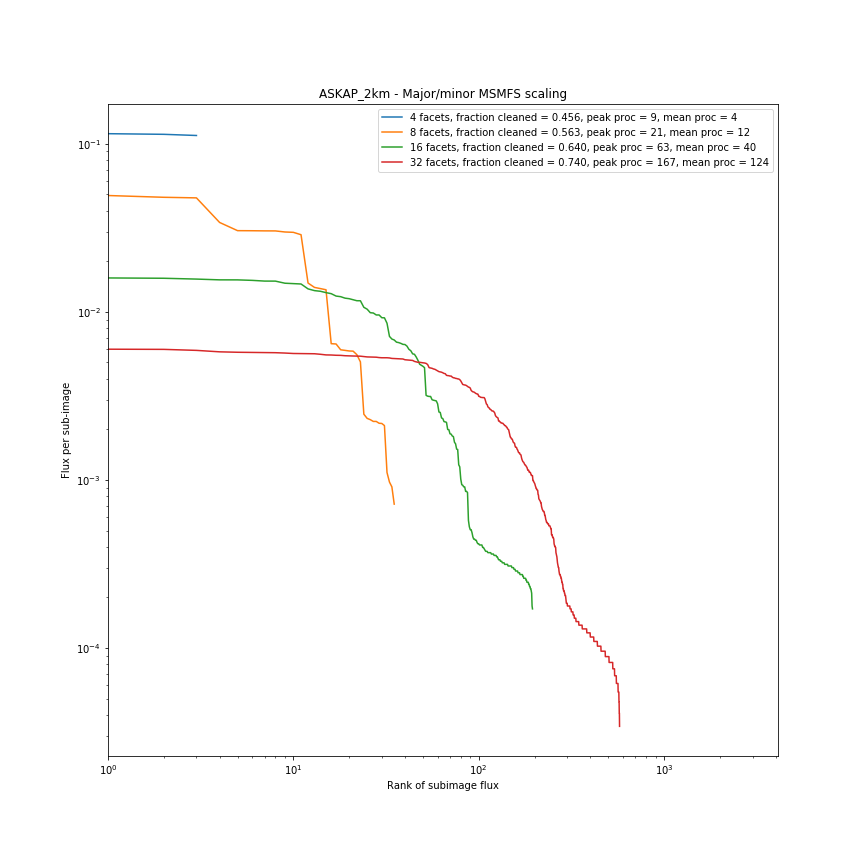
\includegraphics[width=\textwidth]{./aggregate_scaling_ASKAP_2km.png}
  \caption{Aggregate scaling curve for 2km ASKAP configuration. Fraction of flux versus rank for various numbers of facets, for realistic image (constructed from S3-SEX) with a primary beam applied and then clipped at 1mJy/beam. Scales are [0, 3, 10], and the overlap is 16 pixels.}
  \label{fig:aggregate_scaling_2km}
\end{figure}

We have repeated this calculation for the full 36 antenna 6km ASKAP (see figure \ref{fig:aggregate_scaling_6km}).

\begin{figure}[H]
  \centering
  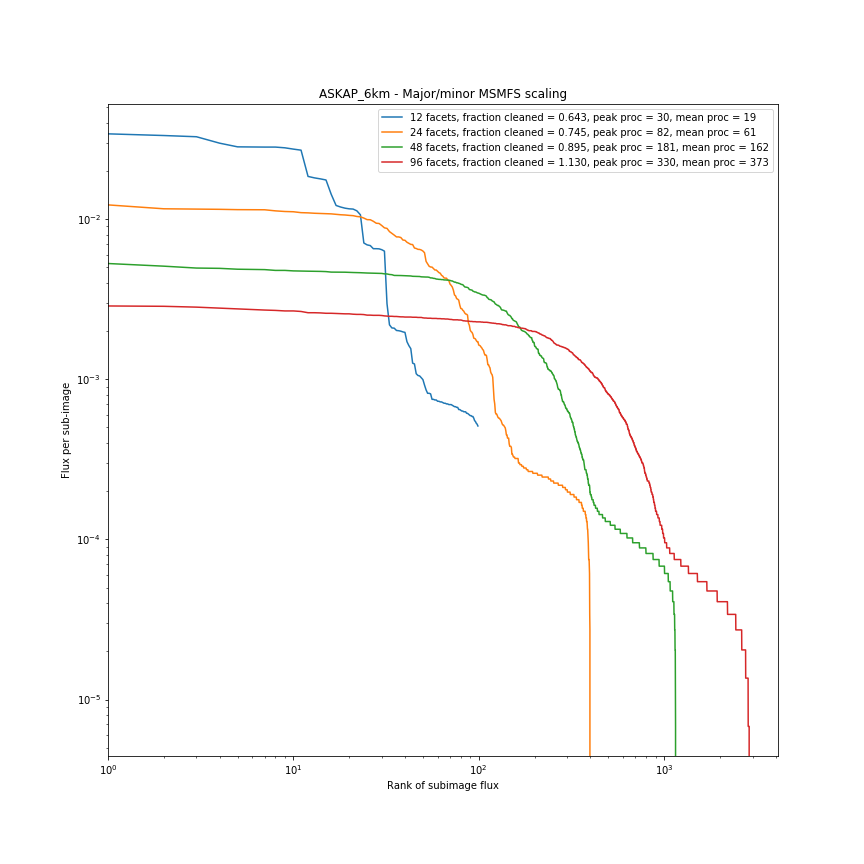
\includegraphics[width=\textwidth]{./aggregate_scaling_ASKAP_6km.png}
  \caption{Aggregate predicted scaling curve for 6km configuration. Fraction of flux versus rank for various numbers of facets, for realistic image (constructed from S3-SEX) with a primary beam applied and then clipped at 1mJy/beam. Scales are [0, 3, 10, 30], and the overlap is 48 pixels.}
  \label{fig:aggregate_scaling_6km}
\end{figure}

\pagebreak
\section{Simulations}
\label{sec:simulations}

The Algorithm Reference Library\footnote{https://github.com/SKA-ScienceDataProcessor/algorithm-reference-library} was used for investigations. The ARL distributes imaging processing using the Dask library\footnote{http://dask.pydata.org}. Since the ARL is python-based, the absolute processing times are not to be taken as realistic for ASKAPsoft, but we use only the relative times in our analysis. 
	
We made simulations as follows:
\begin{itemize}
	\item ASKAP antennas in 2km configuration, 
	\item 11 frequencies spread from 0.85GHz to 1.15GHz, enabling fitting of  Taylor series up to 5 terms (quintic). The bandwidth is sufficiently broad that over the frequency range far out sources can appear and disappear at different frequencies. Hence 5 terms are used for many investigations.
	\item The model was generated by querying the S3-SEX database\footnote{http://s-cubed.physics.ox.ac.uk/s3\_sex}, with a flux cutoff at 10uJy/beam. The spectral index was derived from the 1400MHz and 610MHz fluxes.
	\item Integrations spaced at 12 minutes, no noise added,
	\item Field center at ra=+30deg, dec=-60deg,
	\item Primary beam of 12m antenna with 2m blockage, no feed-legs.
	\item For some simulations the w term was set to zero to concentrate on the cleaning timing.
\end{itemize}

Figure \ref{fig:ASKAP_sim_restored} shows a typical restored image obtained by running 5 major cycles MSMFS with 3 Taylor terms. The residual image (\ref{fig:ASKAP_sim_residual}) shows emission out into the first lobe of the primary beam.

\begin{figure}[H]
  \centering
  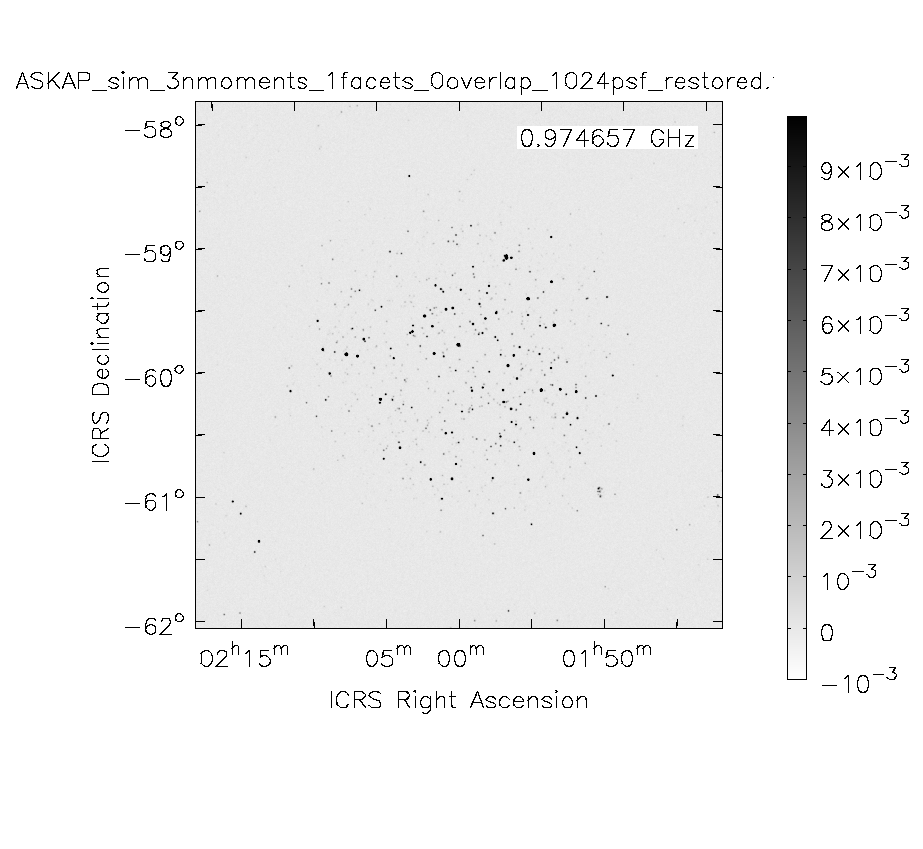
\includegraphics[width=\textwidth]{./ASKAP_sim_restored.png}
  \caption{Test field imaged with the MSMFS, major/minor cycle algorithm in the ARL. The fit is to the first three Taylor terms (i.e. quadratic). No faceting has been used for this image and the PSF support is to the entire field.}
  \label{fig:ASKAP_sim_restored}
\end{figure}

\begin{figure}[H]
  \centering
  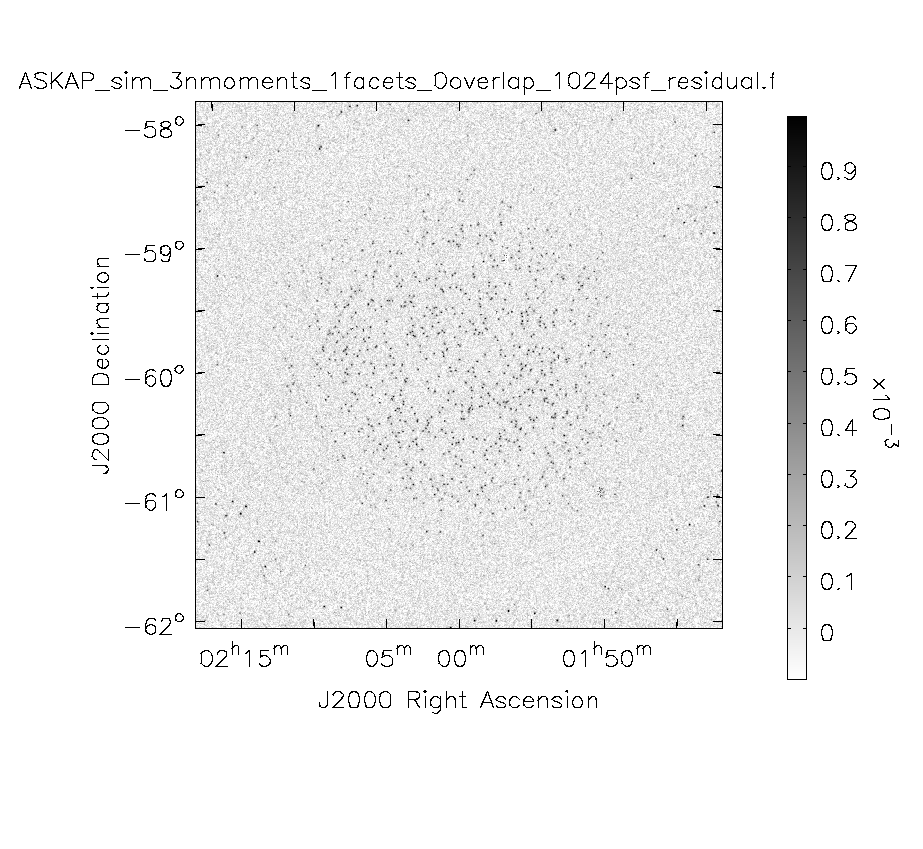
\includegraphics[width=\textwidth]{./ASKAP_sim_residual.png}
  \caption{Residual for test field imaged with the MSMFS, major/minor cycle algorithm in the ARL. The fit is to the first three Taylor terms (i.e. quadratic). No faceting has been used for this image and the PSF support is to the entire field.}
  \label{fig:ASKAP_sim_residual}
\end{figure}

A typical result is shown in figures \ref{fig:ASKAP_sim_restored} (restored image) and \ref{fig:ASKAP_sim_residual} (residual image).

\subsection{Number of facets, and overlap}


\subsection{PSF support}

For a single iteration in the minor cycles, the processing breaks down into a search, scaling as the number of pixels, and a subtraction scaling as the product of the number of pixels in the image and the size of the PSF support. The value of the PSF support used thus directly affects the processing time. Furthermore, the processing via sub-image inevitably means that a limit PSF support will be used.

For the simulated case, the RMS side-lobes of the synthesized beam are about 0.3\% or less for pixels more than a few beams from the PSF peak. Hence we have reason to be optimistic that small values of PSF support will be acceptable given that we use a major/minor cycle. It is therefore important to determine the relationship is between final image quality and the PSF support. 

We investigated the impact of limit PSF support using the simulations described above. In figure \ref{fig:error_vs_support}, we show the fractional error between the images obtained with the restricted PSF and the full PSF as a function of the support. The curve shows that the the effects of limited PSF support are much less than the criterion to switch to a major cycle (typical 10\% or less).

The corresponding run times (wall clock) are shown in figure \ref{fig:time_vs_support}. The scaling is as expected: for small supports, the time is roughly independent of the PSF support, whereas for larger values, the scaling steepens as the component subtraction comes to dominated.

Clearly, small PSF support should be used: the speedup is significant and there is no significant increase in error. As a corollary, the use of sub-images in the deconvolution should be acceptable within a major/minor cycle algorithm.

\begin{figure}[H]
  \centering
  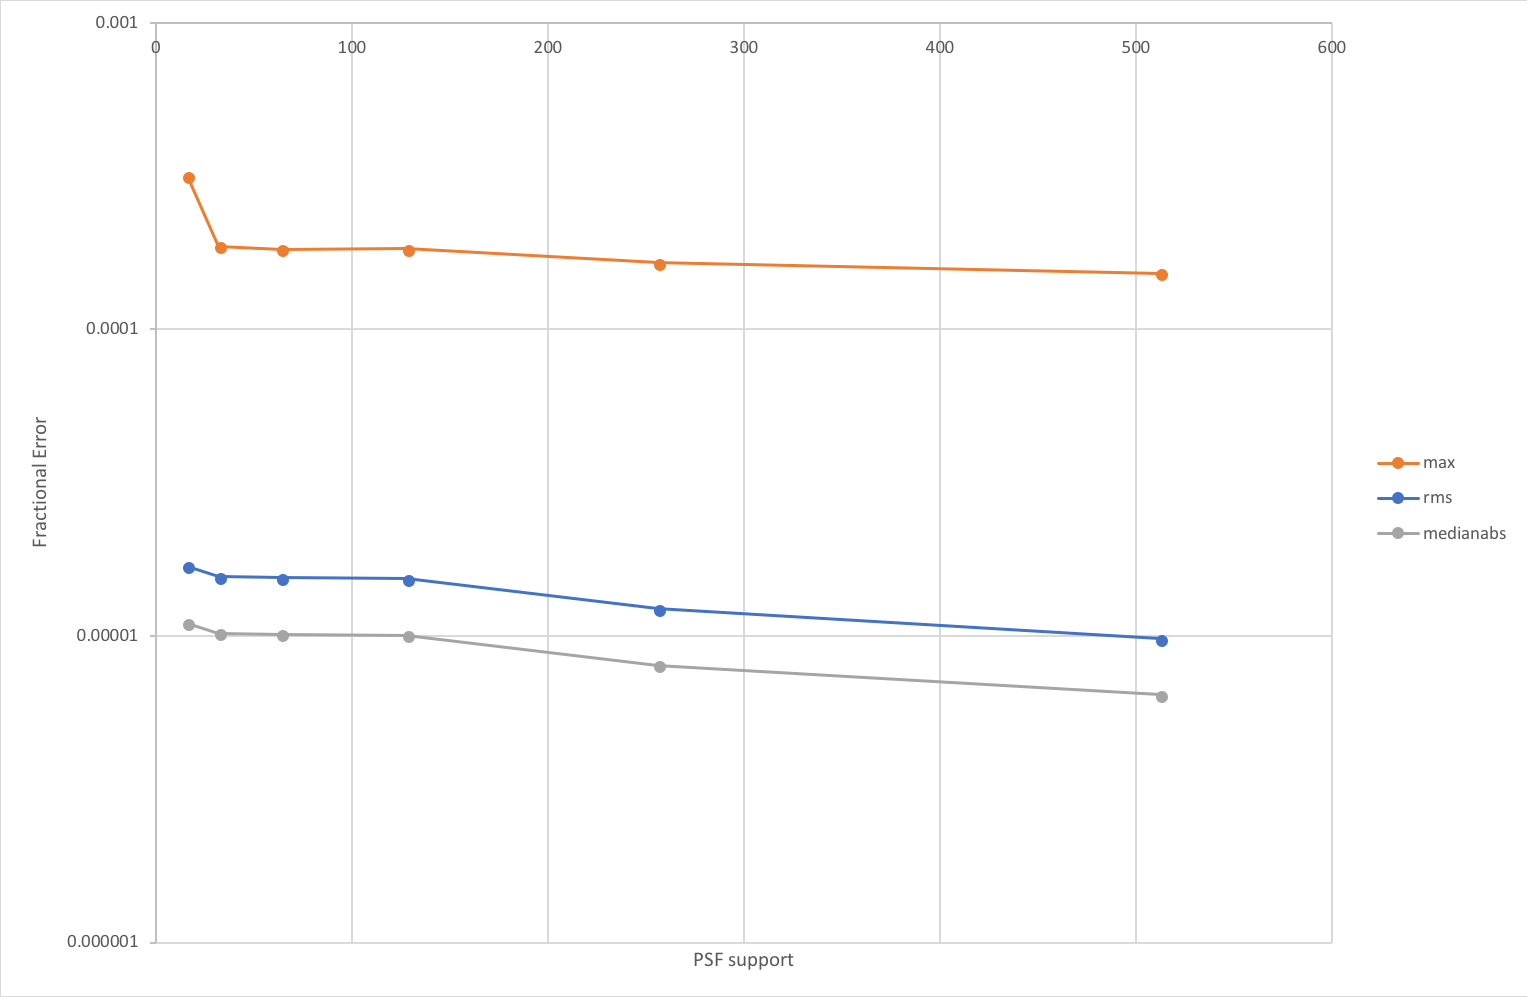
\includegraphics[width=\textwidth]{./error_versus_support.png}
  \caption{Fractional discrepancy as a function of PSF support. This shows a parallel 2048 by 2048 pixel, 3 term MSMFS clean in ARL. The computer was running 4 Dask workers with 32GB each. The discrepancy is the difference between the image processed with PSF support and the image processed with PSF support set to cover the entire image.}
  \label{fig:error_vs_support}
\end{figure}

\begin{figure}[H]
  \centering
  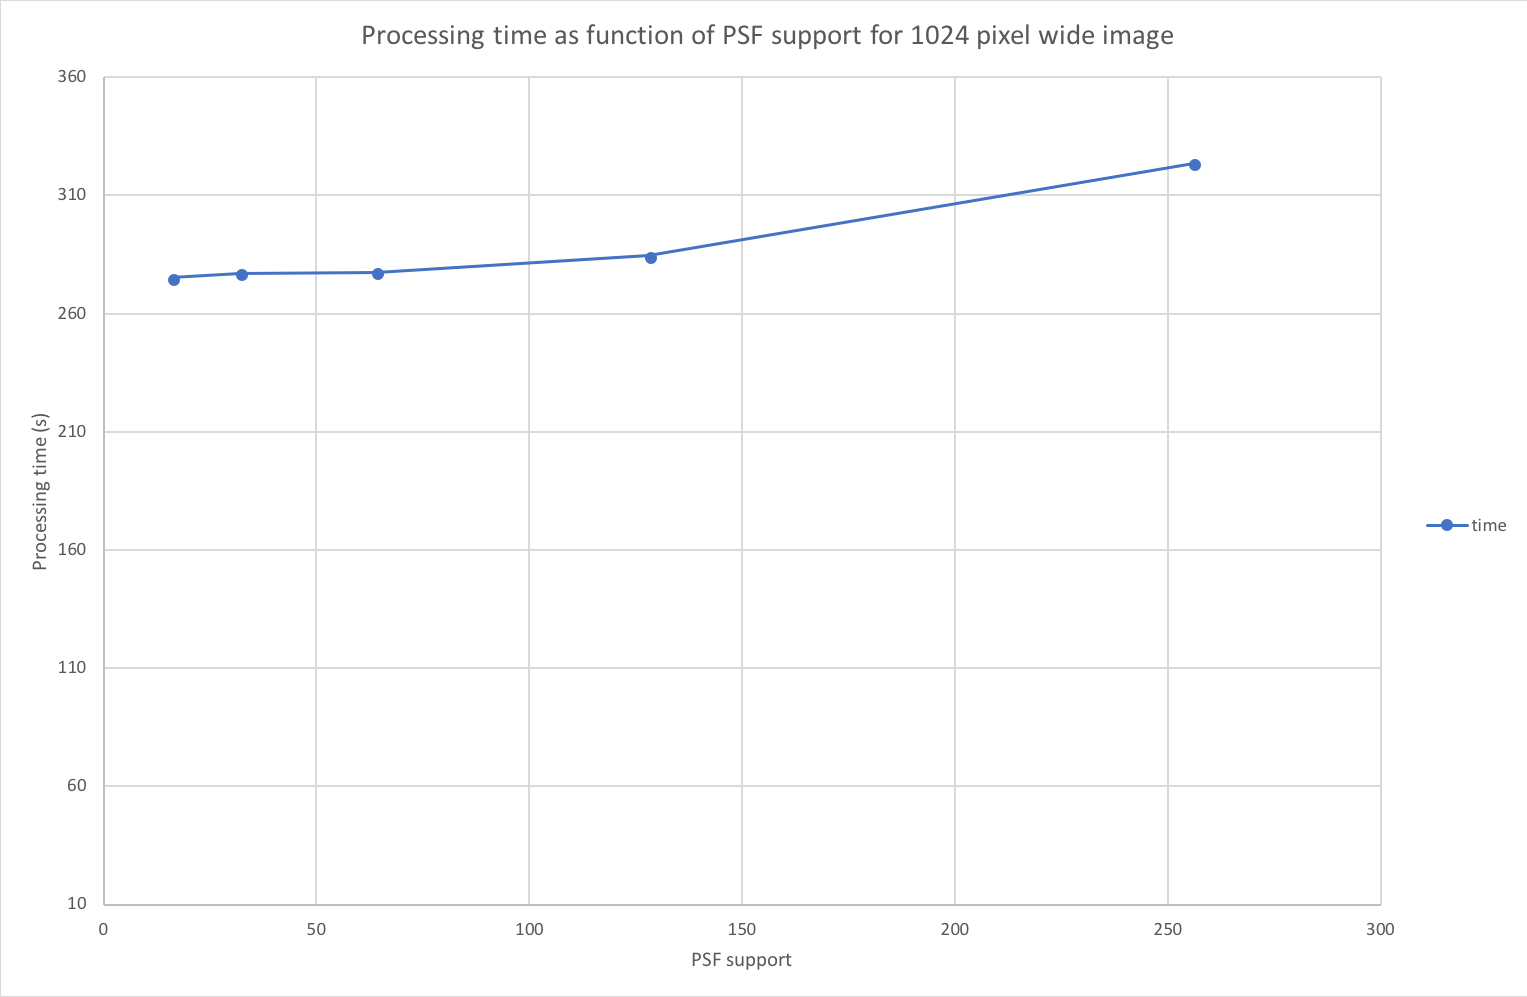
\includegraphics[width=\textwidth]{./time_versus_support}
  \caption{Processing time (seconds) as a function of PSF support. This shows  a parallel 1024 by 1024 pixel, 3 term MSMFS clean in ARL. The computer was running 4 Dask workers with 32GB each.}
  \label{fig:time_vs_support}
\end{figure}


\subsection{Distribution of residuals}

Do the residuals for no overlap and overlap have similar distributions?

\subsection{Spatial structure induced by partitioning}

Do the residuals show excess power on the scale of the overlap?

\pagebreak
\section{Porting to MPI}

For distributed processing, ASKAPsoft uses a master/worker pattern implemented using MPI. In the imager, the master apportions calculation of the normal equations (essentially the residual images) to the workers, gathers and sums the results, and performs a full image single threaded deconvolution using MSMFS. The updated model is then broadcast to all workers, and processing repeats with the new model. Different frequency channels are assigned to different workers. Forming and summing the normal equations is a reduction across the entire set of workers.

Since the scaling curves are relatively flat (see e.g.figures \ref{fig:aggregate_scaling} and \ref{fig:aggregate_scaling_6km}), most processors will be kept close to fully busy while the most demanding (rank 0) case will be processing. Load balancing would then only be needed for the high rank tail.

\pagebreak
\section{Work plan}

\pagebreak
\section{Conclusions}

\begin{enumerate}
	\item We have analysed the performance of the current single threaded MSMFS algorithm in ASKAPSoft. According to the SKA Parametric Model as adapted to ASKAP, the processing can consume anything in the range 30\% - close to 100\%
	\item The motivation for a distributed algorithm is therefore clear. We have developed and demonstrated a distributed MSMFS algorithm that tiles the image space into partially overlapping sub-images and runs the single-threaded MSMFS on each sub-image. The sub-images are then appropriately combined back into a single final image cube, using a Tukey tapering function to reconcile the overlap regions.
	\item This algorithm has been implemented in the SKA Algorithm Reference Library. The distribution of the processing is performed using a graph-based approach.
	\item We have performed an analysis of the large N scaling of this algorithm. The scaling is ultimately determined by the number of sub-images that can be used without distorting the multi-scale deconvolution. For the ASKAP 2km configuration using scales of 0, 3, 10 pixels, this translated to about 32 - 64 sub-images (per axis). For the initial deconvolution cycles, the processing is limited to a few bright sub-images and the strong scaling is limited to 3 - 10 processors. However, as the algorithm proceeds deeper, the sources to be deconvolved occupy more of the image and so more sub-images are active, allowing strong scaling up to 30 - 100 processors. On aggregate, the algorithm shows strong scaling up to 50 - 100 processors (32 - 64 sub-images per axis with 16 pixel overlap).
	\item For the 6km configuration strong scaling is predicted for up to 100 to 300 processors.
	\item This algorithm does not preclude the use of parallelization, such as OpenACC or CUDA to speed up the single sub-image MSMFS. As the speed of the MSMFS processing of a single sub-image improves, the overall speed should improve. 
	\item The flatness of the scaling up to a few hundred processors. There will still need to be some work distribution to deal with the tail in the scaling curves. However, this should fit naturally into the master/worker paradigm used in ASKAPsoft.
\end{enumerate}


% Add the bibliography
\clearpage 

\addcontentsline{toc}{section}{References}
%\bibliography{your_bibfile}%



\end{document}

%%% Local Variables: 
%%% mode: latex
%%% TeX-master: t
%%% End: 
